%%%%%%%%%%%%%%%%%%%%%%%%%%%%%%%%%%%%%%%%%%%%%%%%%%%%%%%%%%%%%%%%%%%%%%%%%%%%%%%%
%%%%%%%%%%%%%%%%%%%%%%%%%%%%%%%%%%%%%%%%%%%%%%%%%%%%%%%%%%%%%%%%%%%%%%%%%%%%%%%%
%%% Template for AIMS Rwanda Assignments         %%%              %%%
%%% Author:   AIMS Rwanda tutors                             %%%   ###        %%%
%%% Email: tutors2018-19@aims.ac.rw                               %%%   ###        %%%
%%% Copyright: This template was designed to be used for    %%% #######      %%%
%%% the assignments at AIMS Rwanda during the academic year %%%   ###        %%%
%%% 2018-2019.                                              %%%   #########  %%%
%%% You are free to alter any part of this document for     %%%   ###   ###  %%%
%%% yourself and for distribution.                          %%%   ###   ###  %%%
%%%                                                         %%%              %%%
%%%%%%%%%%%%%%%%%%%%%%%%%%%%%%%%%%%%%%%%%%%%%%%%%%%%%%%%%%%%%%%%%%%%%%%%%%%%%%%%
%%%%%%%%%%%%%%%%%%%%%%%%%%%%%%%%%%%%%%%%%%%%%%%%%%%%%%%%%%%%%%%%%%%%%%%%%%%%%%%%


%%%%%% Ensure that you do not write the questions before each of the solutions because it is not necessary. %%%%%% 

\documentclass[12pt,a4paper]{article}

%%%%%%%%%%%%%%%%%%%%%%%%% packages %%%%%%%%%%%%%%%%%%%%%%%%
\usepackage{amsmath}
\usepackage{amssymb}
\usepackage{amsthm}
\usepackage{amsfonts}
\usepackage{graphicx}
\usepackage[all]{xy}
\usepackage{tikz}
\usepackage{verbatim}
\usepackage[left=2cm,right=2cm,top=3cm,bottom=2.5cm]{geometry}
\usepackage{hyperref}
\usepackage{caption}
\usepackage{subcaption}
\usepackage{psfrag}

%%%%%%%%%%%%%%%%%%%%% students data %%%%%%%%%%%%%%%%%%%%%%%%
\newcommand{\student}{Yusuf Brima}
\newcommand{\course}{Partial Differential Equations}
\newcommand{\assignment}{2}

%%%%%%%%%%%%%%%%%%% using theorem style %%%%%%%%%%%%%%%%%%%%
\newtheorem{thm}{Theorem}
\newtheorem{lem}[thm]{Lemma}
\newtheorem{defn}[thm]{Definition}
\newtheorem{exa}[thm]{Example}
\newtheorem{rem}[thm]{Remark}
\newtheorem{coro}[thm]{Corollary}
\newtheorem{quest}{Question}[section]

%%%%%%%%%%%%%%  Shortcut for usual set of numbers  %%%%%%%%%%%

\newcommand{\N}{\mathbb{N}}
\newcommand{\Z}{\mathbb{Z}}
\newcommand{\Q}{\mathbb{Q}}
\newcommand{\R}{\mathbb{R}}
\newcommand{\C}{\mathbb{C}}

%%%%%%%%%%%%%%%%%%%%%%%%%%%%%%%%%%%%%%%%%%%%%%%%%%%%%%%555
\begin{document}

%%%%%%%%%%%%%%%%%%%%%%% title page %%%%%%%%%%%%%%%%%%%%%%%%%%
\thispagestyle{empty}
\begin{center}
\textbf{AFRICAN INSTITUTE FOR MATHEMATICAL SCIENCES \\[0.5cm]
(AIMS RWANDA, KIGALI)}
\vspace{1.0cm}
\end{center}

%%%%%%%%%%%%%%%%%%%%% assignment information %%%%%%%%%%%%%%%%
\noindent
\rule{17cm}{0.2cm}\\[0.3cm]
Name: \student \hfill Assignment Number: \assignment\\[0.1cm]
Course: \course \hfill Date: \today\\
\rule{17cm}{0.05cm}
\vspace{1.0cm}
\section*{Question 1}
\begin{enumerate}
		\item[(a)] To compute the full Fourier series representation of
				\begin{equation}
					f(x)=e^{ax}, \quad -\pi\le x< \pi.
					\label{eq:1}
				\end{equation}
			when extended as a $2\pi$-periodic function.\\\ \\
			The general form of a full Fourier series is of the form: 
					\begin{align}
							f(x) &= \frac{a_0}{2} \sum_{n=0}^\infty a_n\cos(nx) + b_n\sin(nx)
							\label{eq:2}
					\end{align}

The Fourier coefficients $a_0, a_n, b_n$ are solved as follows:\\
\begin{align*}
	a_0 &= \frac{1}{\pi}\int_{-\pi}^{\pi} f(x)dx\\
\end{align*}
By substituting the given function in \eqref{eq:1} into the above expression we get:
\begin{align*}
  	a_0 &=\frac{1}{\pi}\int_{-\pi}^{\pi}e^{ax}dx\\
	a_0 &=\frac{1}{\pi}\frac{1}{a}\left[e^{ax}\right]_{-\pi}^{\pi}\\
	a_0 &=\frac{2}{a\pi}\frac{\left(e^{a\pi}-e^{-a\pi}\right)}{2}\\
	a_0 &=\frac{2}{a\pi}\sinh(a\pi)
\end{align*}
For $a_n$\\
\begin{align*}
    a_n &=\frac{1}{L}\int_{-L}^{L}f(x)\cos\left(\frac{n\pi x}{L}\right)dx
\end{align*}
By substituting \eqref{eq:1} into $a_n$\\
\begin{align*}
      a_n &=\frac{1}{\pi}\int_{-\pi}^{\pi}e^{ax}\cos(nx)dx
\end{align*}
We let 
\begin{align*}
		 P=\int_{-\pi}^{\pi}e^{ax}\cos(nx)dx\
\end{align*}
Using Integration by Parts method where:
\begin{align*}
		\int  uv =  uv - \int v du
\end{align*}
Therefore 
$u=e^{ax}  ,\quad  du=ae^{ax}  \quad dv=\cos(nx)dx,\quad  v =\frac{1}{n}\sin(nx)$\\
So 
\begin{align*}
P &=\frac{1}{n}e^{ax}\sin(nx) -\frac{a}{n}\int e^{ax}\sin(nx) dx
\end{align*}
We further integrate 
\begin{align*}
   P_1=\int e^{ax}\sin(nx)dx
\end{align*}
Using Integration by parts as follows\\
where $ u=e^{ax}, \quad du=ae^{ax} \quad dv=\sin(nx)dx, \quad v=\frac{-1}{n}\cos(nx)$\\

\[P_1=\frac{-1}{n}e^{ax} \cos(nx) + \frac{a}{n} \int e^{ax}\cos(nx)dx\]

Therefore,  we can rewrite $P$  as follows: 
\begin{align*}
 P &=\frac{1}{n}e^{ax}\sin(nx)+ \frac{a}{a^2}e^{ax}\cos(nx)-\left(\frac{a^2}{n^2}\right)P\\
P+\left(\frac{a^2}{n^2}\right)P&=\frac{a}{n^2}\left[\frac{1}{n}e^{ax}\sin(nx)+ \frac{a}{a^2}e^{ax}\cos(nx)\right]_{-\pi}^{\pi}\\
P\left( 1 + \frac{a^2}{n^2}\right)&=\frac{a}{n^2}\left[e^{a\pi}\cos(n\pi) - e^{-a\pi}\cos(n\pi)\right]\\
P(n^2+a^2)&=2a(-1)^{n}\left(\frac{e^{a\pi}-e^{-a\pi}}{2}\right)\\
P &=\frac{2a(-1)^{n}}{n^{2}+a^{2} }\sinh(a\pi)
\end{align*}
Finally, the solution for $ a_n $ is: \\
\begin{align*}
a_n &=P (\frac{1}{\pi})\\
a_n &=\frac{1}{\pi}  \frac{2a(-1)^{n}}{ (n^{2}+a^{2} )} \sinh(a\pi)
\end{align*}
We solve for coefficient $b_n$ as follows:\\
\begin{align*}
		 b_n &=\frac{1}{L}\int_{-L}^{L}f(x)\sin\left(\frac{n\pi x}{L}\right)
\end{align*}
By similarly substituting \eqref{eq:1} into the above expression\\
\begin{align*}
  b_n  &=\frac{1}{\pi}\int_{-\pi}^{\pi} e^{ax}\sin(nx)dx
\end{align*}

By substitution, we let  
\[P =\int_{-\pi}^{\pi}e^{ax}\sin(nx)dx\]
And using Method of Integration by Parts where $u=e^{ax} , \quad du=ae^{ax} \quad dv=\sin(nx)dx,\quad v=\frac{-1}{n}\cos(nx)$\\
\begin{align*}
 P  &=\frac{-1}{n}e^{ax}\cos(nx)+\frac{a}{n}\int e^{ax}\cos(nx)dx\\
P &=\frac{-1}{n}e^{ax}\cos(nx)+\frac{a}{n}\left(\frac{1}{n}e^{ax}\sin(nx)-\frac{a}{n}P\right)\\
P &=\frac{-1}{n}e^{ax}\cos(nx)+\frac{a}{n^2}e^{ax}\sin(nx)-\frac{a^2}{n^2}P\\
P\left(1+\frac{a^2}{n^2}\right) &=\left[\frac{-1}{n}e^{ax}\cos(nx)\right]_{-\pi}^{\pi}\\
P\left(1+\frac{a^2}{n^2}\right) &=\frac{-1}{n}\left(e^{a\pi}\cos(n\pi)-e^{-a\pi}\cos(n\pi)\right)\\
P\left(1+\frac{a^2}{n^2}\right) &=\frac{-2}{n}(-1)^{n}\sinh(a\pi)\\
P &=\frac{-2n(-1)^n}{a^2+n^2}\sinh(a\pi)\\
\end{align*}
Therefore, the solution for coefficient  $b_n$ is thus:\\
\begin{align*}
b_n &=\frac{2n(-1)^{n+1}}{\pi(a^2+n^2)}\sinh(a\pi)
\end{align*}
Finally,  all the coefficients into equation \eqref{eq:2}, we therefore get the Fourier solution thus:
\begin{align*}
		f(x)=\frac{1}{a\pi}\sinh(a\pi)+\sum_{n=1}^{\infty}\frac{1}{\pi}\frac{2a(-1)^{n}}{(a^{2}+n^{2} )}\sinh(a\pi)\cos(nx)+ \frac{2n(-1)^{n+1}}{\pi(a^2+n^2)}\sinh(a\pi)\sin(nx)
\end{align*}
\item[(b)] By using the result of equation \eqref{eq:1},  to determine the full Fourier series
expansion for the function
	\begin{equation}
			g(x)=\sinh(x),  \quad \text{ where }  -\pi\le x < \pi
			\label{eq:3}
	\end{equation}

The function in \eqref{eq:3}  can be restated as:\\
\begin{align*}
	\sinh(x)=\frac{e^{x}-e^{-x}}{2}
\end{align*}
We proceed by setting $a = 1$,  and therefore find the Fourier Series for $e^x$ in the expression below.\\
\begin{align*}
	e^x &=\frac{1}{\pi}\sinh(\pi)+\sum_{n=1}^{\infty}\frac{1}{\pi}\frac{2(-1)^{n}}{n^{2}+1 }\sinh(\pi)\cos(nx) + \frac{2n(-1)^{n+1}}{\pi(n^2+1)}\sinh(\pi)\sin(nx)
\end{align*}
And for $e^{-x}$,  we get:\\
\begin{align*}
e^{-x}=\frac{1}{\pi}\sinh(\pi)+\sum_{n=1}^{\infty}\frac{1}{\pi}\frac{2(-1)^{n}}{n^{2}+1 }\sinh(\pi)\cos(nx)- \frac{2n(-1)^{n+1}}{\pi(n^2+1)}\sinh(\pi)\sin(nx)
\end{align*}
Finally,
\begin{align*}
g(x) &=\frac{e^{x}-e^{-x}}{2}=\sum_{n=1}^{\infty}\frac{2n(-1)^{n+1}}{\pi(n^2+1)}\sinh(\pi)\sin(nx)
\end{align*}
\end{enumerate}

\section*{Question 2}
The vibrations $u(x, t)$ of air in an open pipe of unit length satisfy the wave equation 
\begin{equation}
\label{eqn3}
	\frac{1}{c^2} \frac{\partial^2 u}{\partial t^2}  	= \frac{\partial^2 u}{\partial x^2}  \quad 0\le x \le1,\quad \text{and } t>0
\end{equation}
given the boundary conditions
\begin{equation}
\label{equ4}
		\frac{\partial u}{\partial x}(0,t)=0,\frac{\partial u}{\partial x}(1,t)=0,\quad for\quad all \quad 		0\le x \le1
\end{equation}
And the air is initially at rest so that
\begin{equation}
\label{eqn5}
\frac{\partial u}{\partial t}(x,0)=0 \quad for\quad all \quad 0\le x \le1
\end{equation}

\begin{enumerate}
	\item[(a)] We solve the Wave Equation \eqref{eqn3} by Separation of Variables using the Boundary Conditions \eqref{equ4} and Initial Condition \eqref{eqn5}  to show that the solution is:
	\begin{align*}
			 y(x,t)=\sum_{n=0}^{\infty}A_n\cos(n\pi x)\cos(cn\pi t)
	\end{align*}
	as follows:
	\\
	By using the the ansatz $u(x,t)=X(x) T(t)$ we get the following expression.\\
	 \[\frac{1}{c^2}X\ddot{T}=TX^{''}\]
 we divide both sides by $XT$, which results in
 \[\frac{\ddot{T}}{c^{2}T}=\frac{X^{''}}{X}=\lambda\]
 where $\lambda$ is the eigenvalue constants.
 
 We get the following system of differential equations 
\begin{align*}
\ddot{T}-  c^2 \lambda T=0\\
X^{''}-\lambda X=0
\end{align*}
Therefore,
\begin{align*}
\frac{\partial u}{\partial x}(0,t) &=X^{'}(0)T(t)=0\\
\frac{\partial u}{\partial x}(1,t) &=X^{'}(1)T(t)=0
\end{align*}
The non-trivial solution $X^{'}(0)=0$,$X^{'}(0)=0$\\

So we let,  $\lambda_n=-(n\pi)^2$

Solving for $X^{''}-\lambda x=0$ , the characteristic equation is thus:
\begin{align*}
m^{2}+(n\pi)^2 &=0\\
m &=\pm(n\pi i)
\end{align*}
$\implies$
\begin{align*}
X_n(x) &=A_n\cos(n\pi x)+B_n\sin(n\pi x)\\
X_n(x) &=A_n\cos(n\pi x)
\end{align*}

Solving for $\ddot{T}-  c^2 \lambda T=0$ characteristic equation is as follows:
\begin{align*}
m^2+c^2(n\pi)^2 &=0\\
m&=\pm (icn\pi)
\end{align*}
$\implies$
\begin{align*}
T_n(t) &=A_n\cos(cn\pi t)+B_n\sin(cn\pi t)\\
\dot{T_n}(t) &=-cn\pi A_n\sin(cn\pi t)+cn\pi B_n\cos(cn\pi t)\\
\dot{T_n}(0)  &= 0
\end{align*}
Given that
\begin{align*}
\dot{T_n}(0) &=0\Rightarrow B_n =0\\
T_n(t) &=A_n\cos(cn\pi t)\\
\end{align*}
Therefore
\begin{align*}
u(x,t)=\sum_{n=0}^{\infty}A_n\cos(n\pi x)\cos(cn\pi t)
\end{align*}
\item[(b)] We find the \textbf{unique} solution that satisfies the initial condition	:
\begin{align*}
u(x,0)=\begin{cases}
1 \quad for \quad0\le x\le \frac{1}{2}\\
0 \quad for \quad\frac{1}{2}<x\le1
\end{cases}
\end{align*}
as follows:\\

Given that the function is \textbf{even} where $b_n = 0 \implies $
\begin{align*}
u(x,0) &=p(x)=\sum_{n=0}^{\infty}A_n\cos(n\pi x)\\
&=A_0+\sum_{n=1}^{\infty}A_n\cos(n\pi x)
\end{align*}

We solve for the coefficient $A_0$
\begin{align*}
 A_0 &=\frac{2}{2}\int_{0}^{1}p(x)dx=\int_{0}^{1}u(x,0)dx\\
&=\int_{0}^{\frac{1}{2}}1dx+\int_{\frac{1}{2}}^{1}0dx\\
A_0 &=\frac{1}{2}
\end{align*}

And for the coefficient $A_n$
\begin{align*}
A_n &=2\int_{0}^{1}p(x)\cos(n\pi x)dx\\
&=2\left[\int_{0}^{1}\cos(n\pi x)dx+\int_{\frac{1}{2}}^{1}0dx\right]\\
&=\frac{2}{n\pi} \left[  \sin \left( \frac{\pi}{2}n\right)  \right] 
\end{align*}
It follows that 

\[A_n=\begin{cases}
\frac{2}{n\pi}(-1)^{n},\quad n  \text{ is odd} \\
0, \qquad  \quad n  \text{ is even}
\end{cases}\]

Finally,

\[u(x,t)=\frac{1}{2}+\frac{2}{\pi}\sum_{n=1}^{\infty}\frac{(-1)^{2n-1}}{2n-1}\cos(n\pi x)\cos(cn\pi t)\]
\end{enumerate}

\section*{Question 3}
The function $f(x)$ is defined as
\begin{equation}
    f(x) =1 \quad 0<x<\pi  
    \label{eq:05}
\end{equation}
\begin{enumerate}
	\item[(a)] Sketch the odd extension and show that the Fourier sine series expansion is
		\begin{equation}
			\label{eqn:6}
			f(x)=\frac{4}{\pi}\sum_{n=1}^{N}\frac{\sin((2n-1)x}{2n-1}
		\end{equation}
		We determine the coefficient $b_n$ as thus:
		
		\begin{align*}
				b_n &=\frac{2}{\pi}\int_{0}^{\pi}\sin(nx)\\
				&=\frac{2}{\pi}\left[\frac{-\cos(nx)}{n}\right]_{0}^{\pi}\\
				&=\frac{2}{n\pi}\left(1-(-1)^n\right)\\
				b_n&=\begin{cases}
					\frac{4}{n\pi}, \quad   \quad \text{  n is odd}\\
				0 ,  \quad \text{ n is even}
				\end{cases}
		\end{align*}
		\begin{figure}[!h]
			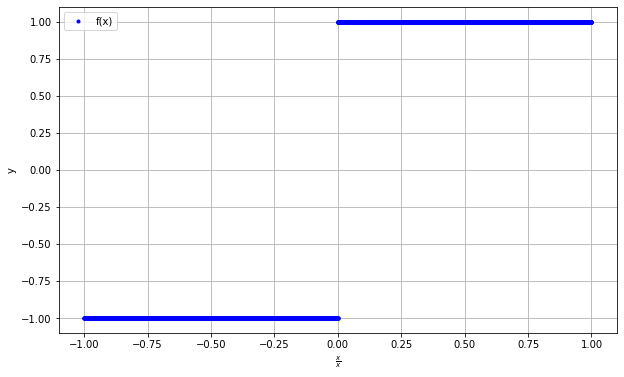
\includegraphics[width=430pt,  height=300pt]{./graphics/q3a1.png}
			\caption{Odd Extension of the $f(x)=1$ from $-\pi \leq x  \leq \pi$}
		\end{figure}
			
			\begin{figure}[!h]
			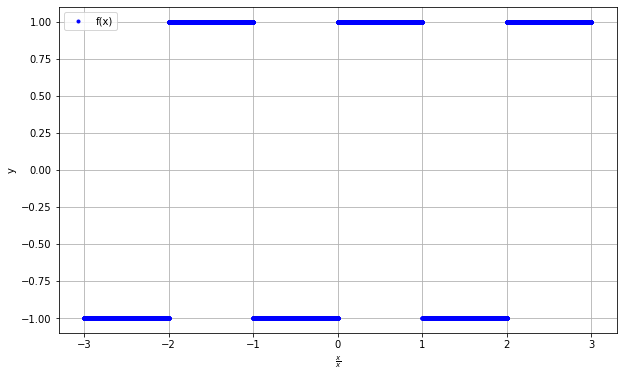
\includegraphics[width=430pt,  height=280pt]{./graphics/q3a2.png}
			\caption{Odd Extension of the $f(x)=1$ from $-3\pi \leq x  \leq 3\pi$}
		\end{figure}
	
	\item[(b)] The graphs of the partial sum plotted in Python are  for equation \eqref{eqn:7}  for the cases when
	$N= 5,10,20,$ over the range $0< x < \pi. $. In addition plot the series with $N= 20,50,500 $
	terms over the range $0< x <0.1$.
	   \begin{equation}
			\label{eqn:7}
		f_N(x)=\frac{4}{\pi}\sum_{n=1}^{N}\frac{\sin((2n-1)x)}{2n-1}
	\end{equation}
	\begin{figure}[!h]
			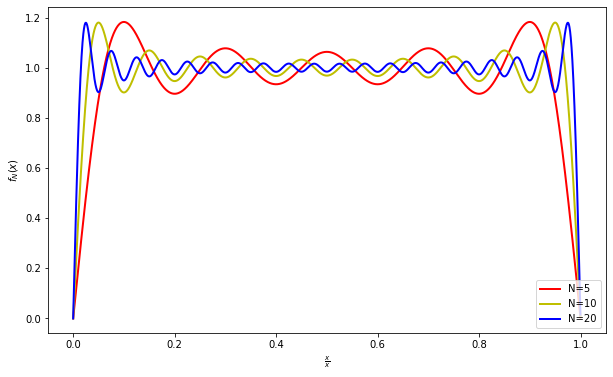
\includegraphics[width=430pt,  height=215pt]{./graphics/q3b1.png}
			\caption{Partial Sums of the Fourier Series from $0  \leq x  \leq \pi$}
		\end{figure}
			\begin{figure}[!h]
			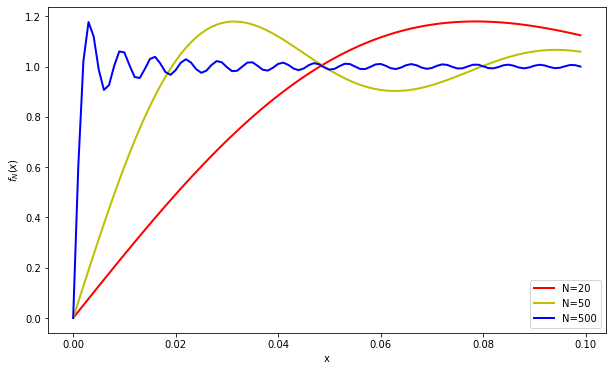
\includegraphics[width=430pt,  height=215pt]{./graphics/q3b2.png}
			\caption{Partial Sums of the Fourier Series from $0  \leq x  \leq \pi$}
		\end{figure}
	\item[(c)] Show that the partial sum in equation \ref{eqn:7} may be written as:
\begin{align*}
f_N(x)=\frac{2}{\pi}\int_{0}^{x}\frac{\sin (2N t)}{\sin (t)}dt
\end{align*}

The following expression can be rewritten as:
\begin{align*}
   \sin\frac{(2n-1)x}{2n-1} &= \int_{0}^{x}\cos((2n-1)t)dt
\end{align*}
Therefore,  we get the following expression:

\begin{equation}
\label{eqn:8}
f_N(x)=\frac{4}{\pi}\left(\sum_{n=1}^{N}\int_{0}^{t}\cos((2n-1)t)\right)dt
\end{equation}

Now when we differential equation \eqref{eqn:8}, we get the following

\begin{equation}
\label{eqn:10}
f_N^{'}(x)=\frac{4}{\pi} \sum_{n=1}^{N}\cos((2n-1)x)
\end{equation}

when we multiply $\sin(x)$ to the above expression in  \ref{eqn:10} we get

\[\sin (x)f_N^{'}(x)=\frac{4}{\pi} \sum_{n=1}^{N}\sin(x)\cos((2n-1)x)\]

Let $P=\cos((2n-1)x)$

 \[P\sin(x)=\sin(x)\cos((2n-1)x)\]
we proceed by using Simpson Formulation 

\[\sin(A) \cos(B) =\frac{1}{2}(\sin(A+B)+\sin(A-B))\]

$\therefore$

\[2P\sin(x)=\sin(x+(2n-1)x)+\sin(x-(2n-1)x)\]
\[=\sin(2nx)-\sin(-2nx+2x)\]
\[=\sin(2nx)-\sin((2-2n)x)\]
\[P\sin(x)=\frac{1}{2}\left(\sin(2nx)-\sin((2-2n)x)\right)\]

We apply summation on both sides as follows $\sin(x)f_N^{'}(x)$
\begin{align*}
\sum_{n=1}^{N}\sin (x)P &=\frac{1}{2}\sin(2Nx)\\
\sum_{n=1}^{N}P &=\frac{1}{2}\frac{\sin(2Nx)}{\sin (x)}\\
\frac{\pi}{4}f_N^{'}(x) &=\frac{1}{2}\frac{\sin(2Nx)}{\sin (x)}\\
\end{align*}
Integrating both sides gives
\begin{align*}
f_N(x) &=\frac{2}{\pi}\int_{0}^{x}\frac{\sin(Nt)}{\sin t} \quad \text{hence proved.}
\end{align*}
\item[(d)]
\end{enumerate}









\end{document}
